% !TeX spellcheck = fr_FR
\chapter{Chapitre 3 : Correspondance avec les données ATLAS-OSM}

Le processus de correspondance entre les données ATLAS et OSM a été conçu pour identifier de manière précise et systématique les arrêts correspondants dans ces deux ensembles de données. Cette approche méthodologique repose sur un principe de correspondance séquentielle par ordre de fiabilité, garantissant une précision maximale des appariements.

\section{Approche méthodologique générale}

Le processus de correspondance adopte une stratégie "hit-first" (première correspondance trouvée), où chaque entrée ATLAS est appariée selon la première méthode qui réussit, en suivant un ordre décroissant de fiabilité. Cette approche séquentielle garantit que les correspondances les plus fiables (exactes) sont privilégiées par rapport aux correspondances moins certaines (par distance).

Nous avons considéré une approche alternative consistant à exécuter toutes les méthodes sur toutes les entrées, permettant d'analyser pour chaque correspondance le nombre de méthodes qui fonctionnent et d'attribuer une probabilité de correspondance. Cependant, après réflexion approfondie, nous avons conclu que cette approche n'apporterait pas de valeur ajoutée significative. En effet, l'ordre séquentiel reflète déjà la hiérarchie de fiabilité : si une correspondance exacte est trouvée, il est inutile de vérifier si d'autres méthodes moins fiables fonctionnent également.

Le processus complet comprend les étapes suivantes :
\begin{enumerate}
    \item \textbf{Correspondance exacte} : Appariement basé sur les identifiants UIC 
    \item \textbf{Correspondance par nom} : Utilisation des noms officiels des arrêts
    \item \textbf{Correspondance par distance} : Analyse géographique avec critères de proximité
    \item \textbf{Correspondance par routes} : Méthode complexe basée sur l'analyse des itinéraires (détaillée au chapitre 4)
    \item \textbf{Consolidation post-traitement} : Récupération des correspondances exactes manquées lors du passage initial
    \item \textbf{Propagation des duplicatas} : Extension des correspondances aux entrées ATLAS dupliquées
    \item \textbf{Correspondance manuelle} : Application des correspondances définies manuellement et stockées de manière persistante
\end{enumerate}

Ce chapitre détaille les méthodes de correspondance manuelle, exacte, par nom et par distance. La correspondance par routes, en raison de sa complexité particulière, sera traitée séparément au chapitre 4.


\section{Correspondance Exacte}

La première étape, appelée correspondance exacte, utilise l’identifiant UIC. Dans les données ATLAS, cet identifiant est représenté par la colonne \texttt{'number'}, tandis que dans OSM, il correspond à la balise \texttt{'uic\_ref'}. Une entrée ATLAS est appariée à un nœud OSM si son \texttt{'number'} est identique au \texttt{'uic\_ref'} du nœud OSM.

Des situations complexes peuvent survenir lorsque plusieurs entrées ATLAS partagent le même \texttt{'number'} (par exemple, plusieurs quais d’une même gare) ou lorsque plusieurs nœuds OSM possèdent le même \texttt{'uic\_ref'}. Pour résoudre ces cas, les règles suivantes sont appliquées :

\begin{enumerate}
    \item \textbf{Cas 1 : Plusieurs entrées ATLAS, un seul nœud OSM}  
    Si plusieurs entrées ATLAS partagent le même \texttt{'number'} et qu’un seul nœud OSM possède ce \texttt{'uic\_ref'}, toutes ces entrées ATLAS sont appariées à ce nœud OSM unique.

    \item \textbf{Cas 2 : Une entrée ATLAS, plusieurs nœuds OSM}  
    Si une seule entrée ATLAS a un \texttt{'number'} donné et que plusieurs nœuds OSM partagent ce \texttt{'uic\_ref'}, tous ces nœuds OSM sont appariées à cette entrée ATLAS unique.

    \item \textbf{Cas 3 : Plusieurs entrées ATLAS et plusieurs nœuds OSM}  
    Lorsque plusieurs entrées ATLAS et nœuds OSM partagent le même \texttt{'number'}/\texttt{'uic\_ref'}, une correspondance plus fine est réalisée en comparant la \texttt{'designation'} de l’entrée ATLAS (par exemple, le code du quai) avec la balise \texttt{'local\_ref'} du nœud OSM. Une correspondance est établie si ces valeurs sont identiques.
\end{enumerate}

Cette méthode a permis d'identifier XX correspondances exactes.
\begin{figure}[h] 
    \centering
    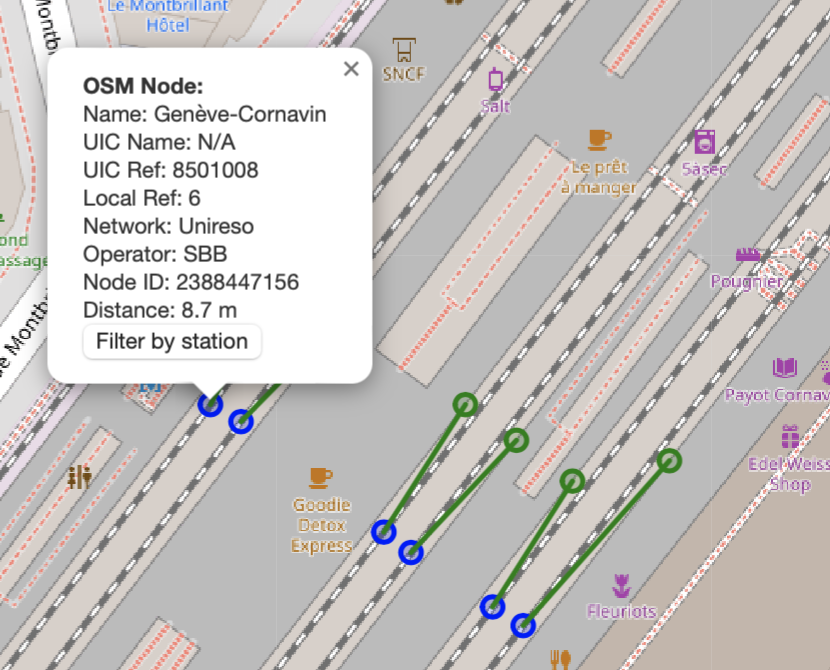
\includegraphics[width=0.7\textwidth]{../figures/correspondances/exact_Cornavin.png}
    \caption[Correspondances exactes à Genève-Cornavin]{Correspondances exactes à la gare de Genève-Cornavin. Les détails du nœud OSM de la voie 6 sont visibles sur l'image.}
    \label{fig:exact_cornavin}
\end{figure}

\section{Correspondance par Nom}

Pour les entrées ATLAS non appariées lors de l’étape précédente, une correspondance basée sur le nom est appliquée. Cette étape compare le nom officiel des arrêts, indiqué dans la colonne \texttt{'designationOfficial'} des données ATLAS, avec plusieurs balises de nom dans OSM : \texttt{'name'}, \texttt{'uic\_name'} et \texttt{'gtfs:name'}.

La règle principale établit une correspondance si le \texttt{'designationOfficial'} correspond exactement à l’une de ces balises OSM. Cependant, si plusieurs nœuds OSM présentent le même nom correspondant, un critère supplémentaire est utilisé : la balise \texttt{'local\_ref'} du nœud OSM est comparée à la \texttt{'designation'} de l’entrée ATLAS. Une correspondance est confirmée si ces valeurs sont identiques (en ignorant la casse).

Cette approche a permis d'ajouter XX correspondances supplémentaires.
\begin{figure}[h]
    \centering
    \begin{subfigure}[b]{0.4\textwidth}
        \centering
        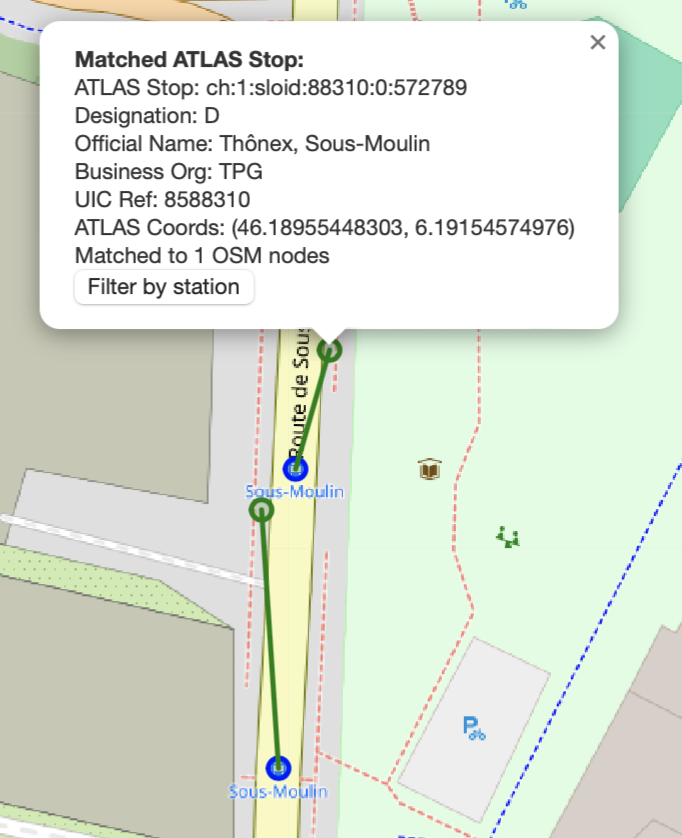
\includegraphics[width=\textwidth]{../figures/correspondances/name_app.png}
        \caption[Correspondances par nom]{Correspondances par nom.}
        \label{fig:name_app}
    \end{subfigure}
    \hspace{-0.2cm}  % Reduce space between images
    \begin{subfigure}[b]{0.45\textwidth}
        \centering
        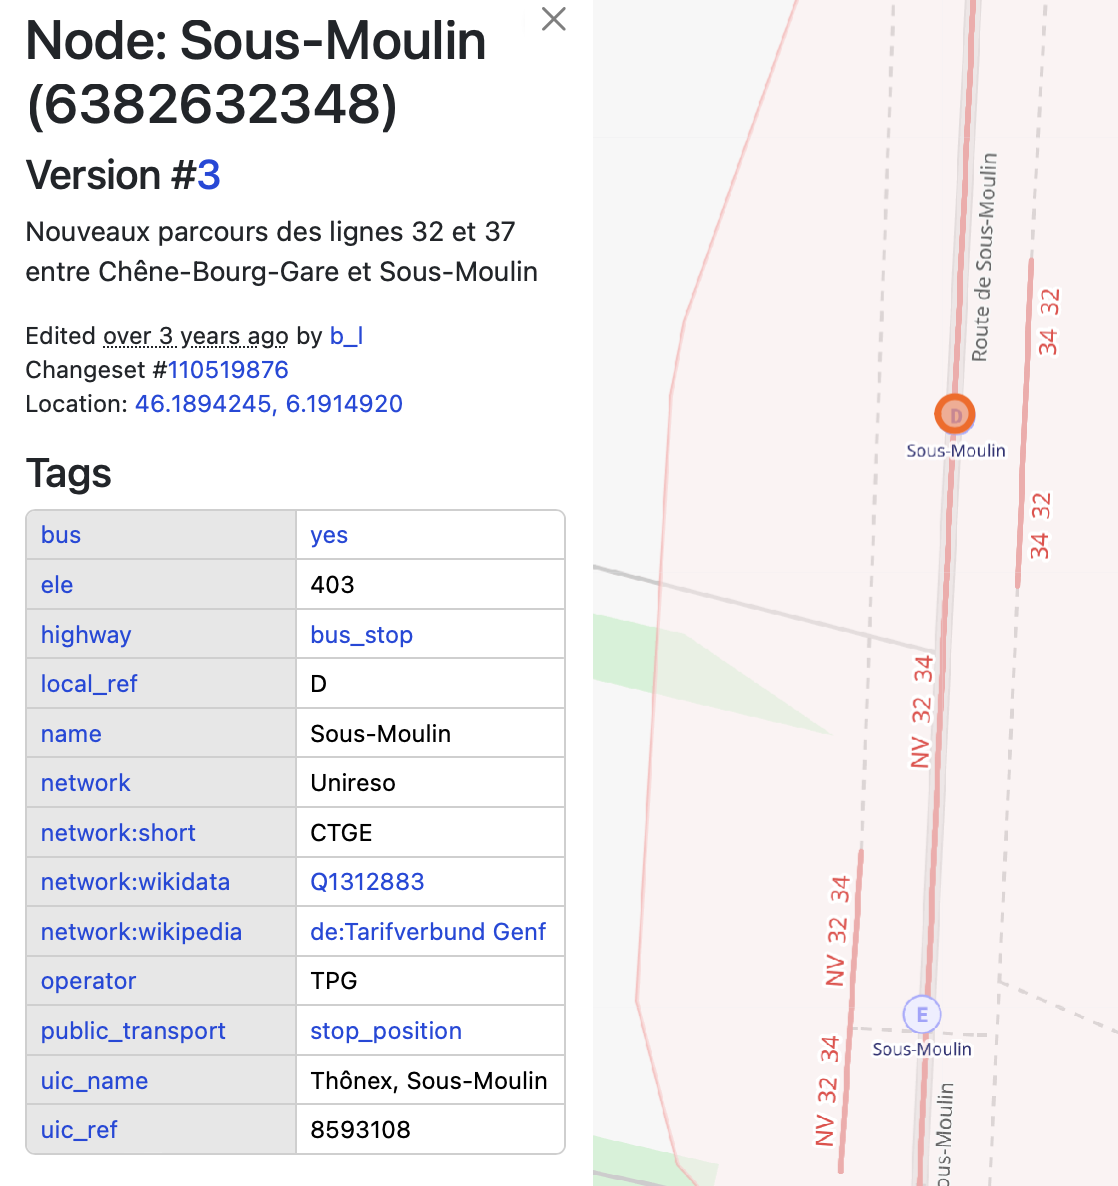
\includegraphics[width=\textwidth]{../figures/correspondances/name_osm.png}
        \caption[Nœud OSM – exemple]{Capture d'écran d'un nœud OSM correspondant.}
        \label{fig:name_osm}
    \end{subfigure}
    \caption[Exemple de correspondance par nom]{Pour l'arrêt "Thônex, Sous-Moulin, D", on peut voir que, malgré une référence UIC différente, il est possible d'établir des correspondances grâce au nom.}
    \label{fig:name_matching_example}
\end{figure}


\section{Correspondance par Distance}

Pour les entrées ATLAS restantes, une correspondance basée sur la proximité géographique est mise en œuvre. Cette étape se divise en trois sous-étapes distinctes, chacune avec des critères spécifiques pour garantir des appariements fiables.

\subsection{Étape 1 : Correspondance de groupe basée sur la proximité}
Les entrées ATLAS et OSM sont regroupés selon les paires d’identifiants suivantes :
\begin{enumerate}
    \item \texttt{'number'} (ATLAS) et \texttt{'uic\_ref'} (OSM).
    \item \texttt{'designationOfficial'} (ATLAS) et \texttt{'uic\_name'} (OSM).
    \item \texttt{'designationOfficial'} (ATLAS) et \texttt{'name'} (OSM).
\end{enumerate}

Dans chaque groupe où le nombre d'entrées ATLAS est égal au nombre de nœuds OSM, une correspondance est tentée en associant chaque entrée ATLAS au nœud OSM le plus proche, à condition que cette association soit cohérente (c'est-à-dire que chaque nœud OSM soit également le plus proche de l'entrée ATLAS qui lui est attribuée). Cette méthode nous a permis de réaliser XX correspondances supplémentaires.

\begin{figure}[h] 
    \centering
    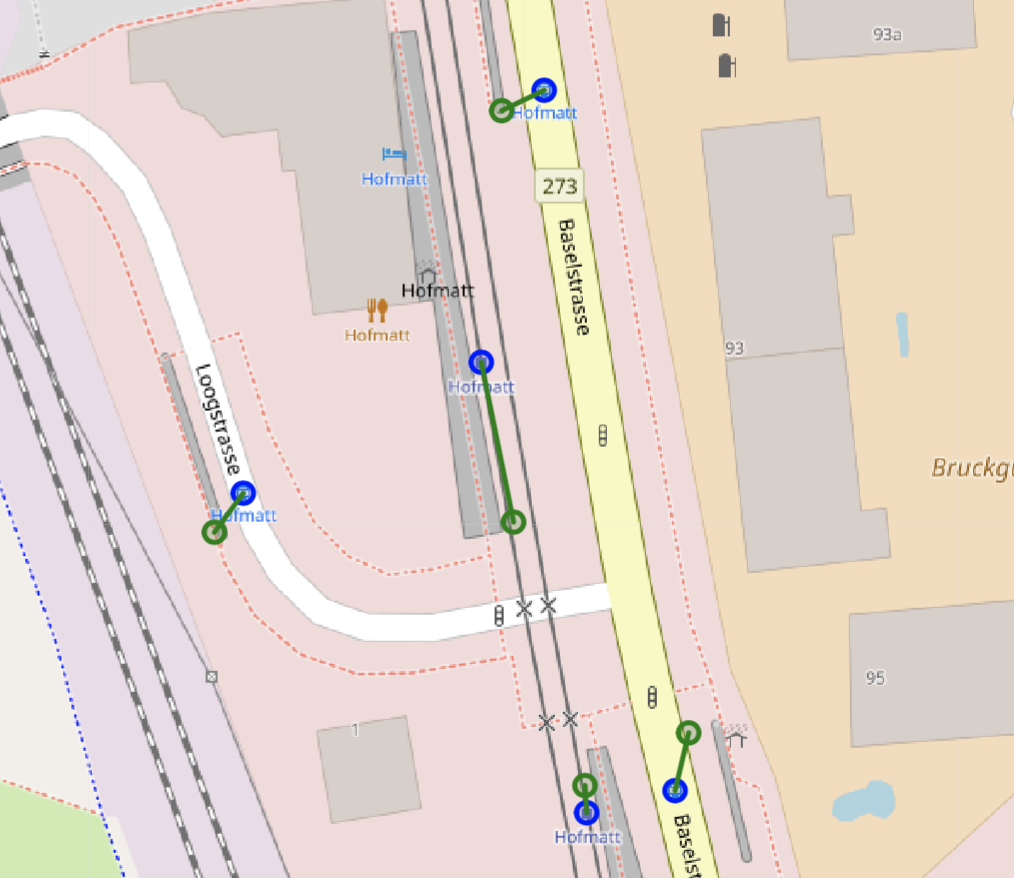
\includegraphics[width=0.7\textwidth]{../figures/correspondances/groupe_proximite.png}
    \caption[Correspondances – Münchenstein, Hofmatt]{Correspondances pour les arrêts de Münchenstein, Hofmatt. Malgré les divergences de \texttt{uic\_ref} et le manque de références locales, nous avons réussi à établir des correspondances grâce à la correspondance de groupe basée sur les distances.}
    \label{fig:group_proximity_munchenstein}
\end{figure}

\FloatBarrier

\begin{table}
\caption[Données ATLAS – Münchenstein, Hofmatt]{Données ATLAS pour les arrêts de Münchenstein, Hofmatt}
\label{tab:atlas_data}
\centering
\begin{tabular}{l l l l l}
\toprule
\texttt{sloid} & \texttt{number} & \texttt{designation} & \texttt{designationOfficial} \\
\midrule
ch:1:sloid:95:1:6 & 8500095 &  & Münchenstein, Hofmatt \\
ch:1:sloid:95:1:5 & 8500095 &  & Münchenstein, Hofmatt \\
ch:1:sloid:95:1:3 & 8500095 &  & Münchenstein, Hofmatt \\
ch:1:sloid:95:1:2 & 8500095 &  & Münchenstein, Hofmatt \\
ch:1:sloid:95:1:1 & 8500095 &  & Münchenstein, Hofmatt \\
\bottomrule
\end{tabular}
\end{table}

\begin{table}[h]
\caption[Données OSM – Münchenstein, Hofmatt]{Données OSM pour les arrêts de Münchenstein, Hofmatt}
\label{tab:osm_data}
\centering
\begin{tabular}{l l l l}
\toprule
\texttt{node\_id} & \texttt{uic\_ref} & \texttt{uic\_name} & \texttt{transport\_type} \\
\midrule
6457499611 & 8578185 & Münchenstein, Hofmatt & bus \\
299126238 & 8500095 & Münchenstein, Hofmatt & tram \\
983964446 & 8578185 & Münchenstein, Hofmatt & bus \\
1435404358 & 8500095 & Münchenstein, Hofmatt & tram \\
3858822225 & 8578185 & Münchenstein, Hofmatt & bus \\
\bottomrule
\end{tabular}
\end{table}

\FloatBarrier

\subsection{Étape 2 : Correspondance par référence locale dans un rayon de 50 mètres}
Cette sous-étape recherche, pour chaque entrée ATLAS non appariée, un nœud OSM situé à moins de 50 mètres dont la balise \texttt{local\_ref} correspond exactement à la \texttt{designation} de l’entrée ATLAS (en ignorant la casse).

À Zürich HB, dans ATLAS, la \texttt{UIC\_ref} est égale à 8503000 pour tous les arrêts, tandis que dans OSM, certains arrêts ont une \texttt{UIC\_ref} de 8516144. 

\begin{figure}[h]
    \centering
    \begin{subfigure}[b]{0.45\textwidth}
        \centering
        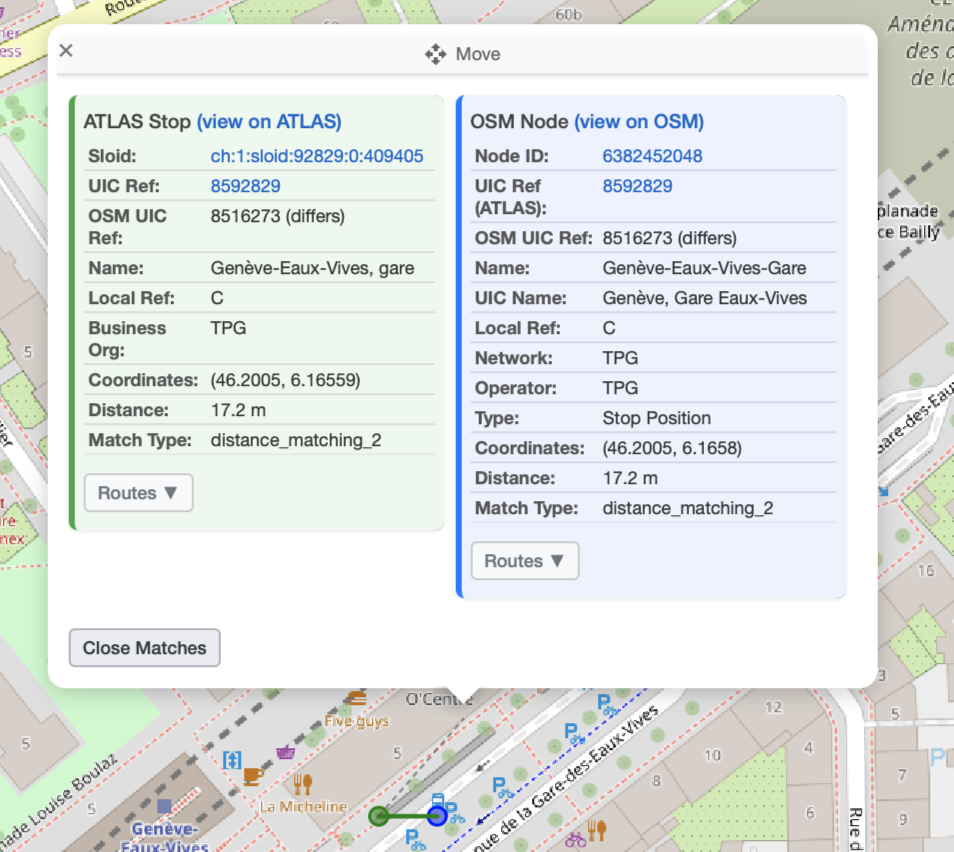
\includegraphics[height=6cm]{../figures/correspondances/distance_2.png}
        \label{fig:zurich_atlas}
    \end{subfigure}
    \hspace{-0.2cm}  % Réduction de l'espace entre les images
    \begin{subfigure}[b]{0.45\textwidth}
        \centering
        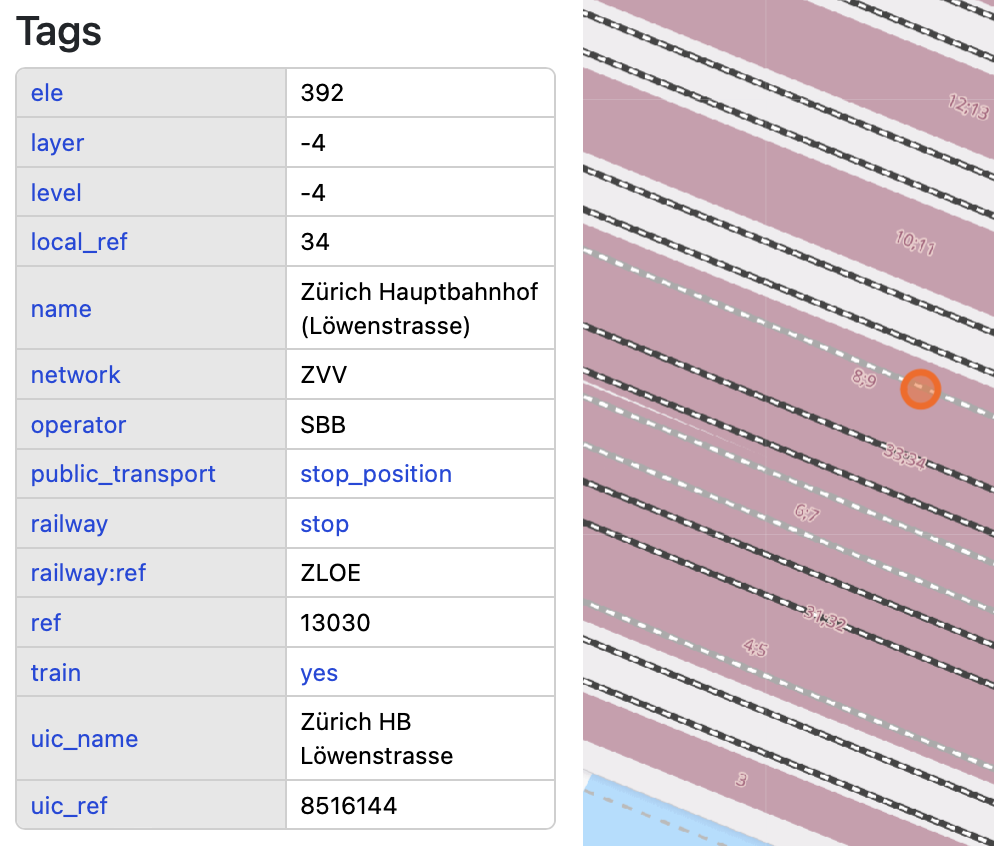
\includegraphics[height=6cm]{../figures/correspondances/osm_distance_2.png}
        \label{fig:zurich_osm}
    \end{subfigure}
    \caption[Correspondances – Zürich HB (étape 2)]{Correspondances à Zürich HB grâce à l'étape 2.}
    \label{fig:zurich_distance_2}
\end{figure}

Cette méthode nous a permis de réaliser XX correspondances supplémentaires.

\subsection{Étape 3 : Correspondance basée sur la proximité avec critères relatifs}  
Pour les entrées toujours non appariées, tous les nœuds OSM situés à moins de 50 mètres sont examinés :  
\begin{itemize}  
    \item a) Si un seul nœud OSM se trouve dans ce rayon, il est apparié à l’entrée ATLAS.  
    \item Si plusieurs nœuds OSM sont présents, l’appariement est effectué avec le nœud le plus proche uniquement si :  
    \begin{enumerate}  
        \item b) Le deuxième nœud le plus proche est à au moins 10 mètres.  
        \item La distance au deuxième nœud le plus proche est au moins 4 fois supérieure à celle du nœud le plus proche.  
    \end{enumerate}  
\end{itemize}  
Nous avons réussi à établir XX correspondances avec l'option a) et XX correspondances avec l'option b).  
Cette méthode est utile pour les cas où il y a des nœuds isolés, comme des télésièges.  

\begin{figure}[h] 
    \centering
    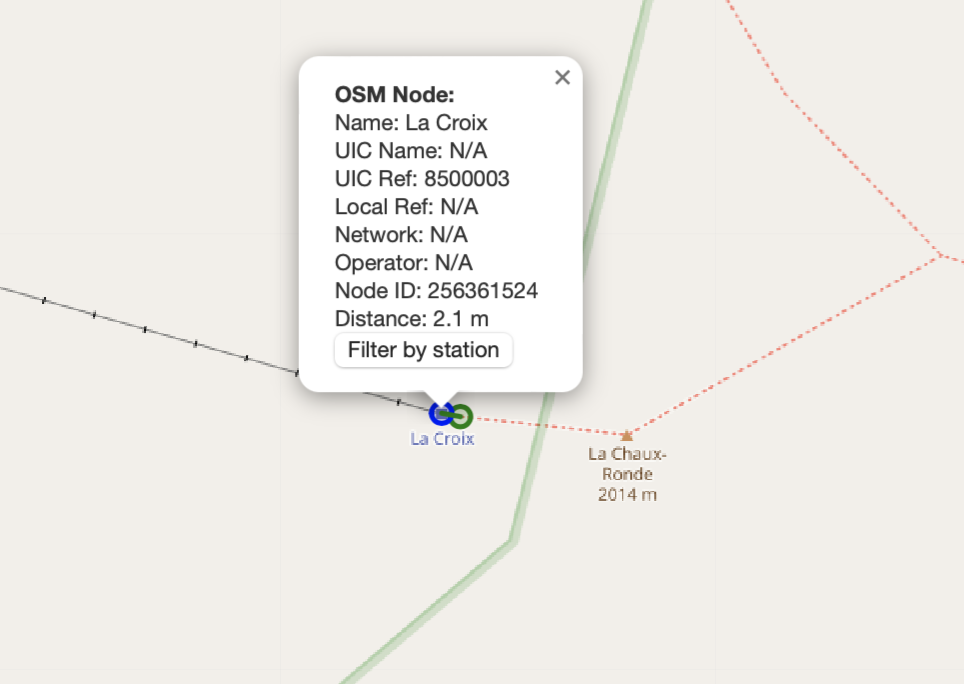
\includegraphics[width=0.7\textwidth]{../figures/correspondances/distance_3.png}
    \caption[Correspondance par distance – étape 3]{Correspondance par distance étape 3 : exemple d'un arrêt isolé où un seul candidat OSM est trouvé dans le rayon de 50 mètres.}
    \label{fig:distance_stage3}
\end{figure} 

\section{Consolidation Post-traitement}

Après l'exécution des méthodes principales de correspondance (exacte, par nom, par distance et par routes), le système effectue une consolidation post-traitement pour récupérer les correspondances exactes qui auraient pu être manquées lors du passage initial. Cette étape, appelée "unique-by-UIC consolidation", examine les entrées ATLAS restantes non appariées et recherche des nœuds OSM disponibles partageant le même identifiant UIC.

Cette consolidation est particulièrement utile dans les cas où :
\begin{itemize}
    \item Des nœuds OSM étaient temporairement indisponibles lors de la correspondance exacte initiale
    \item Des conflits de priorité ont empêché certaines correspondances exactes évidentes
    \item Des entrées ont été filtrées lors des étapes précédentes mais redeviennent candidates valides
\end{itemize}

Le processus fonctionne de manière conservative : il ne crée une correspondance que si exactement un nœud OSM disponible correspond à l'identifiant UIC de l'entrée ATLAS, garantissant ainsi une fiabilité maximale.

Cette étape de consolidation a permis d'identifier XX correspondances exactes supplémentaires.

\section{Propagation des Duplicatas}

Une dernière étape consiste à propager les correspondances trouvées vers les entrées ATLAS dupliquées. Lorsque plusieurs entrées ATLAS partagent les mêmes caractéristiques (numéro et désignation), et qu'une correspondance a été établie pour l'une d'entre elles, cette correspondance est étendue aux autres entrées du groupe dupliqué.

Cette propagation permet d'assurer la cohérence des correspondances et d'améliorer le taux de couverture global, particulièrement dans les grandes gares où plusieurs entrées ATLAS peuvent représenter des aspects différents d'un même arrêt physique.

La propagation des duplicatas a permis d'ajouter XX correspondances supplémentaires.

\section{Correspondance Manuelle}

Enfin, si les entrées n'ont pas été appariées par les méthodes précédentes, le système applique les correspondances manuelles définies préalablement par les utilisateurs et stockées de manière persistante dans la base de données. 

Les correspondances manuelles sont faites depuis l'application web comme on vera plus tard.

\section{Résultats actuels}

Parmi les XX arrêts ATLAS que nous avons considérés, le processus de correspondance a permis d'identifier un total de XX correspondances entre les données ATLAS et OSM, réparties comme suit :

\begin{itemize}
    \item Correspondances exactes : XX
    \item Correspondances par nom : XX
    \item Correspondances par distance : XX
    \begin{itemize}
        \item Étape 1 (groupe-proximité) : XX
        \item Étape 2 (référence locale) : XX
        \item Étape 3a (candidat unique) : XX
        \item Étape 3b (ratio de distance) : XX
    \end{itemize}
    \item Correspondances par routes : XX (détaillé au chapitre 4)
    \item Consolidation post-traitement : XX
    \item Propagation des duplicatas : XX
\end{itemize}

Après ces étapes, XX entrées ATLAS restent non appariées, et XX nœuds OSM restent inutilisés. Parmi ces nœuds OSM inutilisés, XX sont associés à au moins une route, XX possèdent une référence UIC, et XX ont une référence locale (\texttt{local\_ref}).

Parmi les entrées ATLAS non appariées, XX n'ont aucun nœud OSM dans un rayon de 50 mètres, indiquant des zones où la couverture OSM est insuffisante par rapport aux données ATLAS.


